%\documentstyle[epsf,twocolumn]{jarticle}       %LaTeX2e仕様
\documentclass[twocolumn]{jarticle}     %pLaTeX2e仕様(platex.exeの場合)
%\documentclass[twocolumn]{ujarticle}     %pLaTeX2e仕様(uplatex.exeの場合)
%%%%%%%%%%%%%%%%%%%%%%%%%%%%%%%%%%%%%%%%%%%%%%%%%%%%%%%%%%%%%%
%%
%%  基本バージョン
%%
%%%%%%%%%%%%%%%%%%%%%%%%%%%%%%%%%%%%%%%%%%%%%%%%%%%%%%%%%%%%%%%%
\setlength{\topmargin}{-45pt}
%\setlength{\oddsidemargin}{0cm} 
\setlength{\oddsidemargin}{-7.5mm}
%\setlength{\evensidemargin}{0cm} 
\setlength{\textheight}{24.1cm}
%setlength{\textheight}{25cm} 
\setlength{\textwidth}{17.4cm}
%\setlength{\textwidth}{172mm} 
\setlength{\columnsep}{11mm}

\kanjiskip=.07zw plus.5pt minus.5pt


% 【節が変わるごとに (1.1)(1.2) … (2.1)(2.2) と数式番号をつけるとき】
%\makeatletter
%\renewcommand{\theequation}{%
%\thesection.\arabic{equation}} %\@addtoreset{equation}{section}
%\makeatother

%\renewcommand{\arraystretch}{0.95} 行間の設定

%%%%%%%%%%%%%%%%%%%%%%%%%%%%%%%%%%%%%%%%%%%%%%%%%%%%%%%%
\usepackage[dvipdfmx]{graphicx}   %pLaTeX2e仕様(\documentstyle ->\documentclass)\documentclass[dvipdfmx]{graphicx}
\usepackage[dvipdfmx]{color}
\usepackage[subrefformat=parens]{subcaption}
\usepackage{colortbl}
\usepackage{multicol}
%%%%%%%%%%%%%%%%%%%%%%%%%%%%%%%%%%%%%%%%%%%%%%%%%%%%%%%%

\begin{document}

\twocolumn[
\noindent

\hspace{1em}
2020年11月20日
\hfill
\ \ 細川 岳大

\vspace{2mm}

\hrule

\begin{center}
{\Large \bf 進捗報告}
\end{center}
\hrule
\vspace{3mm}
]

% ‚ここから 文章 Start!

\section{今週やったこと}

\begin{itemize}
	%\item optuna
	%\item 予測精度の実験
	\item GAの実験
\end{itemize}

\section{GAの実験}

ラベルなし画像100枚取り出し,それらに対するラベルをGAによって探索する.
表\ref{tb:GApara},\ref{tb:FTXpara}に実験の設定を示す.
遺伝子は0から9の整数値をとる整数値コーディングとした.\\
選択はサイズ2のトーナメント選択,交叉には二点交叉,突然変異は別の数値にランダムに移るように設定した.\\
また,前回trainとevalの分け方を世代ごとに変えるようにした,

\begin{table}[h]
	\centering
	\caption{GAの設定\label{tb:GApara}}
	\scalebox{1.0}{
		\begin{tabular}{|c||c|} \hline
			個体数&30\\ \hline
			世代数&100\\ \hline
			交叉率&1.0\\ \hline
			突然変異率&0.02\\ \hline\hline
			全ラベル付き画像&250枚\\ \hline
			train:eval&100枚:150枚\\ \hline
			search&100枚\\ \hline
		\end{tabular}
	}
\end{table}

\begin{table}[h]
	\centering
	\caption{FixMatchの設定\label{tb:FTXpara}}
	\scalebox{1.0}{
		\begin{tabular}{|c|c|c|} \hline
			model&\multicolumn{2}{c|}{WideResNet28-2}\\ \hline\hline
			data set&\multicolumn{2}{c|}{cifar10}\\ \hline
			train &labeled+serach&200\\ \cline{2-3}
			data&unlabeled&49650\\ \hline
			batch size&labeled+random&64\\ \cline{2-3}
			&unlabeled&$64*7$\\ \hline
			val data&\multicolumn{2}{c|}{150}\\ \hline\hline
			num\_iterations&\multicolumn{2}{c|}{5000}\\ \hline
			optimizer&\multicolumn{2}{c|}{SGD(lr=0.1,momntum=0.9)}\\ \hline
			loss&\multicolumn{2}{c|}{cross\_entropy\_loss}\\ \hline
		\end{tabular}
	}
\end{table}

\subsection{結果}
図\ref{fig:ex1}に示す.
14世代以降でfitnessが落ちてしまっているのはtrainにおいて
もともとのラベル付きデータを入れ忘れてしまっていたからであった.
ただし,それを抜きにしても精度の頭打ちが来ていることが分かる.

\begin{figure}[h]
	\begin{center}
		\vspace*{-3mm}
		\hspace*{-8mm}
		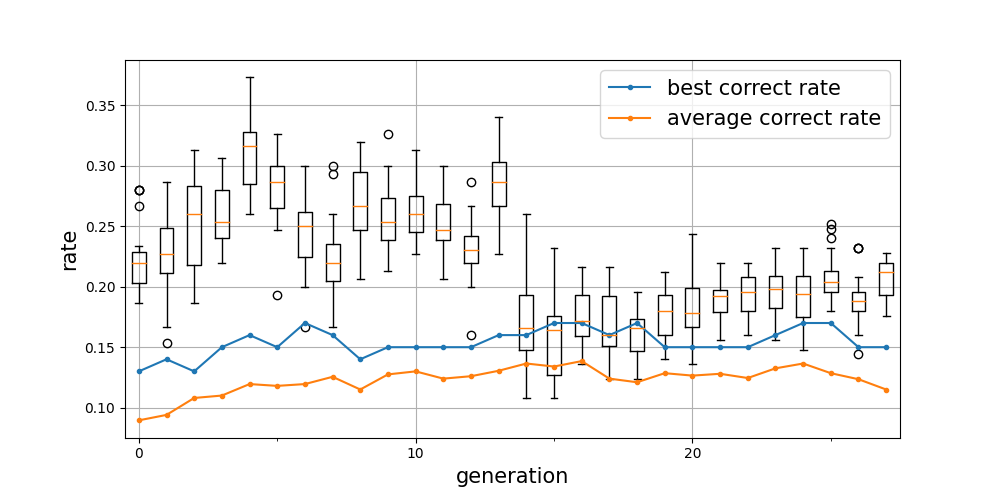
\includegraphics[height=65mm,width=110mm]{graph.png}
		\caption{結果\label{fig:ex1}}
	\end{center}
\end{figure}

\section{SSLの実験}
あるラベルなしデータに各0から9までのラベルをつけて
精度を求め,最も高い精度のラベルをつけてラベル付きデータへと加える
ような実験をした.
表\ref{tb:SVMpara}にSVMの設定を示す.
\begin{table}[h]
	\centering
	\caption{SVMの設定\label{tb:SVMpara}}
	\scalebox{1.0}{
		\begin{tabular}{|c|c|} \hline
			kernel&poly\\ \hline
			C&3.654\\ \hline
			$\gamma$&53.15\\ \hline
			coef0&0.0\\ \hline
			degree&3\\ \hline
		\end{tabular}
	}
\end{table}
また,cifar10使用し,ラベル付きデータ250枚をtrainとvalに100枚:150枚で分けて探索する.

\subsection{まとめ}
時間がなく結果をまとめることができていないが
ポイントとしては以下のものが挙げられた.\\
\begin{itemize}
	\item 大体20\%ほどの正答率であった.
	\item 正答ラベルの時だけがとびぬけて精度が良かったというわけではなかった.
	\item 正誤答関わらず初期の段階でつけられたラベルが同じものが続いたとき,そのあともそのラベルが多く出現する傾向にあった.
\end{itemize}

\section{来週の課題}
	\begin{itemize}
		\item 実験設定の改良
	\end{itemize}


\end{document}


